\chapter{قلت برمجة ؟}

\section{ما هي البرمجة ؟}

\begin{question}
  ما الذي تعنيه كلمة "بَرْمَجَ"؟
\end{question}

لن أتعبك وأعطيك أصل كلمة "بَرْمَجَ"، لكنني سأختصر كل شيء في جملة : البرمجة تعني إنشاء برامج حاسوب. وهذه البرامج التي تنشئها تأمر الجهاز بالقيام بتعليمات وأفعال معيّنة.
حاسوبك الخاص يحتوي على كثير من هذه البرامج وبمختلف أنواعها :

\begin{itemize}
  \item الآلة الحاسبة تعتبر برنامجاً.
  \item معالج النصوص يعتبر برنامجاً أيضاً.
  \item وكذلك برنامج المحادثة.
  \item ألعاب الفيديو هي برامج كذلك.
\end{itemize}

\begin{figure}[H]
	\centering
	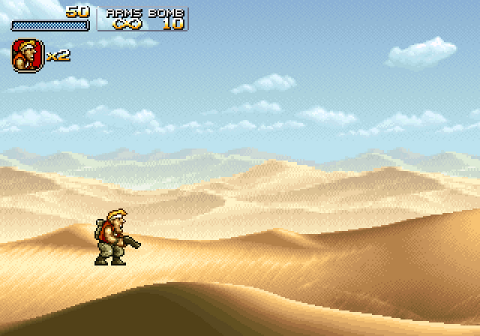
\includegraphics[width=0.8\textwidth]{Chapter_I-1_MetalSlug}
	
نسخة عن لعبة \textenglish{MetalSlug} الشهيرة تم إنشاؤها من طرف العضو \href{http://www.siteduzero.com/membres-294-176405.html}{\textenglish{joe87}}	
\end{figure}

باختصار البرامج موجودة في كل جهاز، وهي التي تعطي الحاسوب قدرته على إنجاز مختلف المهام التي تُخوَّل إليه. يمكنك أن تنشئ برنامج تشفير أو لعبة ثنائية / ثلاثية الأبعاد باستخدام لغة برمجة مثل \textenglish{C}.

ملاحظة : لم أقل أن إنشاء لعبة يتم برمشة عين، لقد قلت فقط بأنه شيء ممكن، لكن كن متأكداً، سوف يتطلب ذلك جهدا كبيراً !

وبما أننا في بداية الطريق، فإّننا لن نقوم بإنشاء لعبة ثلاثية الأبعاد ! لكنّنا سنبدأ بكيفية عرض نص على الشاشة، طبعا ستقول ما علاقة هذا بإنشاء الألعاب ؟ لكن ثِق بي، هذا الأمر ليس بسيطا كما يبدو !

بالطبع هذا ليس شيئا مُبهراً، ولكن يجب علينا أن نبدأ من هنا؛ وشيئا فشيئا يمكنك أن تنشئ برامج معقّدة أكثر. فالهدف من هذا الكتاب هو أن أعرفك على كل ما يتعلق بهذه اللغة.

\section{البرمجة، بأي لغة يا ترى ؟}

حاسوبك هو آلة غريبة جداً، هذا أقل ما يمكن أن نقوله عنه. يمكننا أن نخاطبه فقط بالصفر والواحد، فمثلا إذا طلبنا منه حساب 3+5 فيمكن لهذا أن يعطينا نتيجة كالتالي (هذه ليست ترجمة دقيقة ولكنها تشبه ما يحدث بالفعل):
\InlineCode{0010110110010011010011110}

ما تَرَاه هنا يسمى اللغة الثنائية
(\textenglish{Binary language})
أو لغة الآلة
(\textenglish{Machine language})،
وحاسوبك لا يفهم سوى هذه اللغة، وكما تلاحظ، هذه اللغة غير مفهومة على الإطلاق !

مشكلتنا الآن :

\begin{question}
  كيف يمكننا التعامل مع حاسوب لا يفهم سوى اللغة الثنائية ؟
\end{question}

حاسوبك لا يتحدث الإنجليزية، ولا العربية، ولا أي لغة غير هذه اللغة، ولكنها صعبة جدا لدرجة أن حتى أكبر خبراء الحاسوب لا يستخدمونها.
لهذا قام بعض مهندسي الحواسيب باختراع لغات يمكن أن تُتَرجَمَ إلى اللغة الثنائية، لكن الشيء الأصعب هو إنشاء البرامج الّتي تقوم بهذه الترجمة. ولحسن الحظ فقد قاموا بهذا العمل نيابة عنا. هذه البرامج تقوم بترجمة الأوامر الّتي تكتبها (مثلا : "أُحسب 3+5") إلى شيء يشبه هذا :
\InlineCode{0010110110010011010011110}.

هذا المخطط يلخص ما كنت أشرح :

\begin{figure}[H]
	\centering
	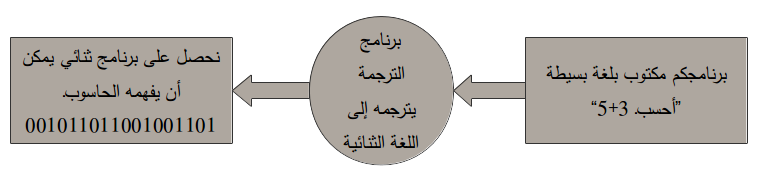
\includegraphics[width=\textwidth]{Chapter_I-1_Translation}
\end{figure}

\section{قليل من المفردات}

حتّى الآن كنت أتحدّث إليك بكلمات بسيطة، لكن يجب أن تعلم أنه في المعلوماتية توجد مصطلحات علمية لكل ما ذكرت. طوال هذا الكتاب، سوف تتعلم استخدام المفردات المناسبة. هذا سيفيدك كثيرا خصوصا عندما تتحدث مع مبرمجين آخرين، حيث أنك سوف تتفاهم معهم بكل سهولة.

نعود إلى الحديث عن المخطط السابق. في المستطيل الأول قلت أن "برنامجك مكتوب بلغة مُبَسَّطة"، في الواقع هذا النوع من اللغات يُعرف باسم لغات البرمجة عالية المستوى (\textenglish{High-level programming languages}). هناك مستويات عديدة من لغات البرمجة، وكلما كان مستوى اللغة أعلى كانت أقرب إلى اللغة الحقيقية وكان استخدامها أسهل. إذن، اللغات عالية المستوى سهلة الاستخدام لكنها تتضمن بعض السلبيّات سوف نتعرّف عليها لاحقا.

توجد العديد من لغات البرمجة، وهي متفاوتة المستوى، منها :
\begin{itemize}
  \item \textenglish{C}
  \item \textenglish{C++}
  \item \textenglish{Java}
  \item \textenglish{Visual Basic}
  \item \textenglish{Delphi}
  \item و العديد غيرها
\end{itemize}

كما تلاحظ، لم أرتبها حسب مستوياتها، لذلك لا تعتقد أن اللغة الأولى في القائمة هي الأسهل أو العكس. عموما، لائحة اللغات الموجودة طويلة جدا لدرجة أنه لا يمكنني كتابتها كلها هنا.

مصطلح آخر يجب تذكّره هو
\textbf{الشفرة المصدرية}
(\textenglish{Source code})،
 وهي ببساطة الشفرة الخاصة ببرنامجك الذي تكتبه بلغة عالية المستوى والذي يتم ترجمته فيما بعد إلى اللغة الثنائية.

 ثم يأتي دور البرنامج الذي يحوّل هذه اللغة عالية المستوى إلى اللغة الثنائية، هذا النوع من البرامج يعرف باسم
 \textbf{المترجم}
  أو
  \textbf{المصنّف}،
 والعملية الّتي يقوم بها تسمى
 \textbf{الترجمة}
 أو
 \textbf{التصنيف}.

\begin{information}
  يوجد لكل لغة عالية المستوى مترجم خاص، وهذا شيء منطقي، فاللغات مختلفة فيما بينها، فلا يمكننا ترجمة لغة
\textenglish{C}
بنفس الطريقة الّتي نترجم بها
\textenglish{Delphi}
مثلا.
  بعض اللغات مثل
\textenglish{C}
تملك العديد من المترجمات، فمنها من هو مكتوب من طرف
\textenglish{Microsoft}
، و منها من
\textenglish{GNU}
، إلخ \dots سوف نتعرّف على كل هذا في الفصل القادم.
  لحسن الحظ، هذه المترجمات متطابقة تقريبا (رغم وجود اختلافات طفيفة بينها سوف نتعرف عليها لاحقا).
\end{information}

أخيرا، البرنامج الثنائي المنشئ بواسطة المترجم يسمى الملف
\textbf{القابل للتنفيذ}
أو
\textbf{التنفيذي}
(\textenglish{Executable}).
 لهذا السبب تملك البرامج
 (على الأقل برامج
 \textenglish{Windows})
 الامتداد
\textenglish{.exe}
 والذي هو اختصار كلمة
 \textenglish{EXEcutable}.

 نعود إلى مخططنا السابق، وهذه المرة سنستخدم المصطلحات الصحيحة :

\begin{figure}[H]
	\centering
	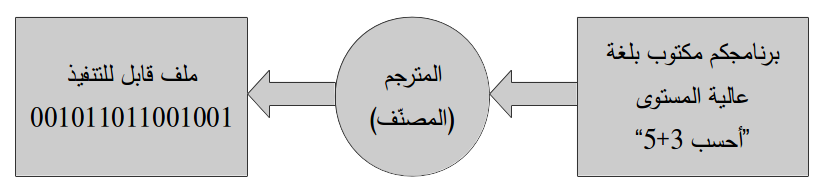
\includegraphics[width=\textwidth]{Chapter_I-1_Compilation}
\end{figure}

 \section{لماذا نختار تعلّم \textenglish{C}؟}
 
 كما قلت سابقا، يوجد كثير من اللغات عالية المستوى، فلماذا ينبغي علينا أن نبدأ بإحداها على وجه الخصوص ؟ سؤال عظيم !

على أية حال يجب علينا أن نختار بأي لغة سنبدأ البرمجة عاجلا أم آجلا، وبالتالي لديك الخيار في البدء بـ :

\begin{itemize}
  \item \textbf{لغة ذات مستوى عالي جدّا} :
 وتكون سهلة جدّا أوعامة، نذكر من بينها
 \textenglish{Python}، \textenglish{Ruby}، \textenglish{Visual Basic}،
 وغيرها. هذه اللغات تسمح بكتابة برامج بشكل أسرع. عامّة تحتاج لأن تُرفق معها ملفات مُسَاعِدة لكي تعمل (كَمُفَسِّرٍ مثلا).
  \item \textbf{لغة ذات مستوى منخفض قليلا} :
هي أكثر صعوبة نوعا ما، ولكن مع لغة مثل
\textenglish{C}
 سوف تتعلم كثيرا عن البرمجة وحول طريقة عمل حاسوبك. ستكون بعد ذلك قادراً على تعلّم لغة برمجة أخرى إن أردت وبكل يُسْرٍ.
\end{itemize}

من ناحية أخرى،
\textenglish{C}
لغة برمجة واسعة الإنتشار، أُستخدمت في برمجة العديد من البرامج التي تعرفها. حتى أنها كثيرا ما تدرّس في الدراسات العليا في مجال المعلوماتية.
هذه هي الأسباب الّتي جعلتني أتحمّس لتعليمك لغة
\textenglish{C}
بالتحديد. لم أقل أنّه يجب عليك أن تبدأ بها، لكنّي قلت إنه خيار جيّد لكي أقدّم لك معرفة صلبة في هذا الكتاب.

\begin{information}
  بعض لغات البرمجة موجّهة أكثر للشبكة العنكبوتية
 (\textenglish{Web})
 مثل
 \textenglish{PHP}
 أكثر منها لإنشاء البرامج المعلوماتية.
\end{information}

سوف أفترض في هذا الكتاب أنّ هذه هي لغة برمجتك الأولى وأنّه لم يسبق لك أن برمجت من قبل. فإن كنت قد برمجت قليلا من قبل فلا مضرّة في أن تعيد من الصفر.

\begin{question}
  ما هو الفرق بين
  \textenglish{C}
  و
  \textenglish{C++}
  ؟
\end{question}

هاتان اللغتان قريبتان جدّا من بعضهما، وكلاهما مستخدمتان بكثرة. ولكي تعرف كيف نشأتا يجب عليك أن تدرس التاريخ قليلا :
\begin{itemize}
  \item في البداية، عندما كانت الحواسيب تَزِنُ أطنانا وتشغل مكانا قَدْرُهُ حجم منزلك، تمّ اختراع لغة برمجة تسمّى
\textenglish{Algol}.
  \item بعدها تطوّرت الأمور أكثر واختُرعَت لغة برمجة جديدة عُرِفَتْ باسْمِ
\textenglish{CPL}
 والّتي تطوّرت فيما بعد إلى لغة
\textenglish{BCPL}
 ثم أخذت إسم اللغة
\textenglish{B}.
  \item مع مضيّ الزمن توصّل الخبراء إلى ابتكار اللغة
\textenglish{C}
 وقد تمّ إدخال بعض التعديلات عليها إلّا أنها لا تزال من أحد اللغات الأكثر استخداما اليوم.
  \item وبعد زمن، أراد الخبراء أن يضيفوا بعض الأشياء إلى
\textenglish{C}
، يمكن اعتبارها نوعا من التحسينات. والنتيجة كانت بما يعرف بلغة
\textenglish{C++}
، وهي لغة
\textenglish{C}
 مع إضافات تمكّننا من البرمجة بطريقة مختلفة.
\end{itemize}

\begin{information}
  الـ\textenglish{C++}
ليست أحسن من الـ\textenglish{C}
، هي فقط تمكننا من البرمجة بطريقة مختلفة وتساعد المبرمج على تنظيم شفرة برنامجه. رغم ذلك هي تشبه الـ\textenglish{C}
كثيرا. وإن كنت تنوي تعلّم الـ\textenglish{C++}
فيما بعد فَسَوْفَ تجد ذلك سهلا.
\end{information}

ولو اعتُبرت
\textenglish{C++}
 تطويرا لـ\textenglish{C}
 فإن هذا لا يعني أنه يجب استخدام
\textenglish{C++}
 فقط لإنشاء البرامج. لغة
\textenglish{C}
 ليست لغة عجوزا منسيّة، بالعكس هي مستخدمة بكثرة اليوم. بل إنها أساس أنظمة التشغيل الكبيرة مثل
\textenglish{Unix }
(ومنه
\textenglish{GNU/Linux}
 و
\textenglish{Mac OS}) و
\textenglish{Windows}.

\section{هل البرمجة صعبة ؟}
هذا سؤال يعذّب روح كل من يريد تعلّم البرمجة ! هل يجب أن تكون أستاذ رياضيات كبير درس 10 سنوات من التعليم العالي حتّى تبدأ البرمجة ؟

الجواب هو لا بالطبع. كل ما تحتاج إليه هو معرفة العمليات الأربع الأساسية :
\begin{itemize}
  \item الجمع
  \item الطرح
  \item الضرب
  \item القسمة
\end{itemize}
هذا ليس مخيفا ! سوف أشرح لك في فصل لاحق كيف يقوم الحاسوب بهذه العمليات الأساسية في برامجك.

باختصار، لا توجد صعوبات غير قابلة للحلّ. في الواقع، هذا يعتمد على طبيعة برنامجك، فإذا كنت تريد إنشاء برنامج تشفير فيجب عليك معرفة بعض الأشياء في الرياضيات، وإن كان برنامجك يقوم بالرسم ثلاثي الأبعاد فيجب أن تكون لديك بعض المعرفة بالهندسة الفضائية.

كل حالة تعامل بطريقة خاصّة. ولكن لتعلّم لغة
\textenglish{C}
 نفسها لا تحتاج إلى أيّة معارف قبليّة.

\begin{question}
  إذن أين هو الفخ ؟ وأين تكمن الصعوبة ؟
\end{question}

يجب أن تعرف كيف يعمل الحاسوب، لتفهم ما الّذي نقوم به في \textenglish{C}. من هذا المنطلق، كن متيقّنا أنّي سأعلّمك كلّ هذا شيئا فشيئا.

اعلم أن للمبرمج صفات أيضا مثل :
\begin{itemize}
  \item الصبر : البرنامج لا يعمل عادة من أوّل محاولة، يجب أن تكون مثابراً.
  \item حسّ المنطق : صحيح أنّك لست بحاجة إلى أن يكون لديك مستوى جيّد في الرياضيّات، لكنّ هذا لا يمنع من التفكير وتحليل المشكلات بالمنطق.
  \item الهدوء : فيجب عليك ألّا تضرب حاسوبك بالمطرقة، فهذا لن يجعل برنامجك يعمل !
\end{itemize}
